\subsection{Appendix: Interpreting Q-Q Plots}

A Quantile-Quantile (Q-Q) plot is a graphical tool used to assess if a dataset follows a specified theoretical distribution, typically the normal distribution. The Q-Q plot compares the quantiles of the sample data to the quantiles of the theoretical distribution. Below is a detailed explanation of how to interpret Q-Q plots:

\subsubsection{Understanding Q-Q Plots}

\begin{itemize}
    \item \textbf{Quantiles}: Quantiles are cut points dividing the range of a probability distribution into continuous intervals with equal probabilities. In a Q-Q plot, the quantiles of the sample data are plotted against the quantiles of a theoretical distribution.
    \item \textbf{Theoretical Distribution}: Often, the theoretical distribution is the normal distribution, but Q-Q plots can be used for other distributions as well.
    \item \textbf{45-Degree Line}: The line y = x (a 45-degree line) represents the ideal scenario where the sample quantiles perfectly match the theoretical quantiles. If the sample data follows the theoretical distribution, the points should fall approximately along this line.
\end{itemize}

\subsubsection{Interpreting the Q-Q Plot}

\begin{itemize}
    \item \textbf{Points on the Line}: If the points lie approximately along the 45-degree line, the sample data likely follows the theoretical distribution.
    \item \textbf{Deviations from the Line}: Deviations from the line indicate departures from the theoretical distribution. The nature of the deviation provides insights into the type of departure.
        \begin{itemize}
            \item \textbf{Heavy Tails}: Points that deviate from the line at the ends (tails) suggest heavier or lighter tails than the theoretical distribution. For instance, if points curve away from the line at the ends, the data may have heavier tails than the normal distribution.
            \item \textbf{Systematic Curvature}: If the points form an S-shaped curve, this may indicate skewness in the data. A leftward (downward) curve suggests left-skewness (negative skewness), and a rightward (upward) curve suggests right-skewness (positive skewness).
            \item \textbf{Outliers}: Individual points that fall far from the line may indicate outliers in the data.
        \end{itemize}
    \item \textbf{Center of the Plot}: Points near the center of the plot (representing the median quantiles) should ideally lie on the line if the central tendency of the data matches the theoretical distribution.
\end{itemize}

\begin{figure}[H]
    \centering
    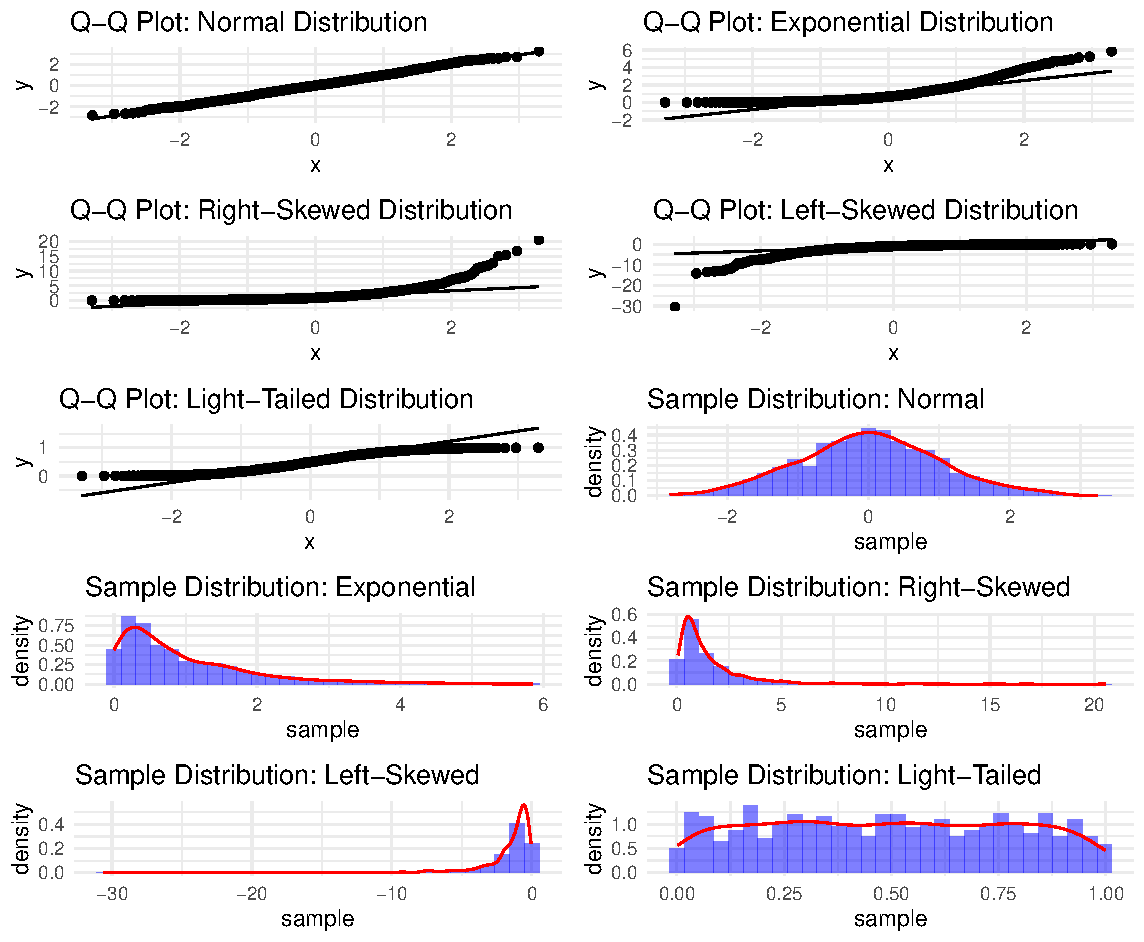
\includegraphics[width=1\textwidth]{plots/Q-QExample.pdf}
    \caption{Q-Q Plot Examples}
\end{figure}